\documentclass{amsart}
\usepackage{amssymb,amsmath,amsthm,mathrsfs,graphics,hyperref,stmaryrd,psfrag,arcs,xypic}
\usepackage[enableskew]{youngtab}
\numberwithin{equation}{section}
\raggedbottom
\oddsidemargin=0in
\evensidemargin=0in
\textwidth=6.5in
\textheight=8.8in
\topmargin=0.25in
\headheight=0in
\headsep=0.2in
\footskip=0in
\parskip=10bp
\parindent=0bp

\newcommand{\excise}[1]{}
\newcommand{\Latex}[1]{\textbackslash\texttt{#1}}

\newcommand{\bigpad}{\rule[-14mm]{0mm}{30mm}}
\newcommand{\smallpad}{\rule[-1.5mm]{0mm}{5mm}}
\newcommand{\pad}{\rule[-3mm]{0mm}{8mm}}
\newcommand{\padup}{\rule{0mm}{5mm}}
\newcommand{\paddown}{\rule[-3mm]{0mm}{2mm}}
\newcommand{\blank}{\rule{1.25in}{0.25mm}}
\newcommand{\commentout}[1]{}
\newcommand{\yell}[1]{\fbox{\rule[-1mm]{0mm}{4mm} \large\bf #1 }}
\newcommand{\bang}{$\bullet$\quad}
\newcommand{\indnt}{\phantom{.}\qquad}
\newcommand{\littleline}{\begin{center}\rule{4in}{0.5bp}\end{center}}

\newcommand{\includefigure}[3]{{
  \begin{center}
  \resizebox{#1}{#2}{\includegraphics{{figs/#3}}}
  \end{center}}}
\newcommand{\includefigurewithinmath}[3]{{
  \resizebox{#1}{#2}{\includegraphics{{figs/#3}}}}}

%\newcommand{\defterm}[1]{\underline{\textbf{#1}}}
\newcommand{\defterm}[1]{\textbf{#1}}

\DeclareMathOperator{\ch}{\mathbf{ch}}
\DeclareMathOperator{\colspace}{colspace}
\DeclareMathOperator{\corank}{corank}
\DeclareMathOperator{\CST}{CST}
\DeclareMathOperator{\deln}{del}
\DeclareMathOperator{\diag}{diag}
\DeclareMathOperator{\ess}{ess}
\DeclareMathOperator{\Gr}{Gr}
\DeclareMathOperator{\Hom}{Hom}
\DeclareMathOperator{\im}{im}
\DeclareMathOperator{\Irr}{Irr}
\DeclareMathOperator{\Ind}{Ind}
\DeclareMathOperator{\Int}{Int}
\DeclareMathOperator{\lcm}{lcm}
\DeclareMathOperator{\link}{lk}
\DeclareMathOperator{\nullity}{nullity}
\DeclareMathOperator{\nullspace}{nullspace}
\DeclareMathOperator{\Poin}{Poin}
\DeclareMathOperator{\proj}{proj}
\DeclareMathOperator{\rank}{rank}
\DeclareMathOperator{\Res}{Res}
\DeclareMathOperator{\Span}{span}
\DeclareMathOperator{\supp}{supp}
\DeclareMathOperator{\row}{row}
\DeclareMathOperator{\rowspace}{rowspace}
\DeclareMathOperator{\sh}{sh}
\DeclareMathOperator{\tr}{tr}
\DeclareMathOperator{\wt}{wt}

\newtheorem{theorem}{Theorem}[section]
\newtheorem{proposition}[theorem]{Proposition}
\newtheorem{lemma}[theorem]{Lemma}
\newtheorem{corollary}[theorem]{Corollary}
\theoremstyle{definition}
\newtheorem{definition}[theorem]{Definition}
\newtheorem{example}[theorem]{Example}
\newtheorem{remark}[theorem]{Remark}
\newtheorem{problem}[theorem]{Problem}


\newcommand{\cor}{{\bf Corollary: }}
\newcommand{\defn}{{\bf Definition: }}
\newcommand{\defns}{{\bf Definitions: }}
\newcommand{\exa}{{\bf Example: }}
\newcommand{\fact}{{\bf Fact: }}
\newcommand{\lem}{{\bf Lemma: }}
\newcommand{\notn}{{\bf Notation: }}
\newcommand{\obs}{{\bf Observation: }}
\newcommand{\note}{{\bf Note: }}
\newcommand{\prop}{{\bf Proposition: }}
\newcommand{\rmk}{{\bf Remark: }}
\newcommand{\thm}{{\bf Theorem: }}

\newcommand{\basecase}{\emph{Base case: }}
\newcommand{\indstep}{\emph{Inductive step: }}
\newcommand{\skpr}{\emph{Sketch of proof: }}

\newcommand{\0}{\emptyset}
\newcommand{\Alt}{\mathfrak{A}}
\newcommand{\Braid}{Br}
\newcommand{\CHI}{\chi^{\phantom{*}}}
\newcommand{\Cl}{C\ell}
\newcommand{\covers}{\gtrdot}
\newcommand{\coveredby}{\lessdot}
\newcommand{\dedge}[1]{\overrightarrow{{#1}}}
\newcommand{\dom}{\rhd}
\newcommand{\domeq}{\unrhd}
\newcommand{\domby}{\lhd}
\newcommand{\dombyeq}{\unlhd}
\newcommand{\Fspan}{\Ff\text{-span}}
\newcommand{\isom}{\cong}
\newcommand{\join}{\vee}
\renewcommand{\Join}{\bigvee}
\newcommand{\Laff}{L^{\text{aff}}}
\newcommand{\lin}[1]{\overleftrightarrow{{#1}}}
\newcommand{\meet}{\wedge}
\newcommand{\Meet}{\bigwedge}
\newcommand{\ov}[1]{\overline{{#1}}}
\newcommand{\partn}{\vdash}
\newcommand{\qqandqq}{\qquad\text{and}\qquad}
\newcommand{\qandq}{\quad\text{and}\quad}
\newcommand{\qand}{\quad\text{and}}
\newcommand{\qbin}[2]{{\begin{bmatrix}#1\\#2\end{bmatrix}_q}}
\newcommand{\sd}{\triangle} % symmetric difference
\newcommand{\simK}{\underset{K}{\sim}} % Knuth equivalence
\newcommand{\simJ}{\underset{J}{\sim}} % jeu de taquin equivalence
\newcommand{\sm}{\setminus}
\newcommand{\st}{~|~}
\newcommand{\soln}{\textit{Solution:\ }}
\newcommand{\Sym}{\mathfrak{S}}
\newcommand{\un}[1]{\underset{*}{#1}}
\newcommand{\unA}{\un{A}}
\newcommand{\unB}{\un{B}}
\newcommand{\unw}{\un{w}}
\newcommand{\unx}{\un{x}}
\newcommand{\uny}{\un{y}}
\newcommand{\unz}{\un{z}}
\newcommand{\x}{\times}

\renewcommand{\aa}{\mathbf{a}}
\newcommand{\bb}{\mathbf{b}}
\newcommand{\nn}{\mathbf{n}}
\newcommand{\pp}{\mathbf{p}}
\newcommand{\qq}{\mathbf{q}}
\newcommand{\xx}{\mathbf{x}}
\newcommand{\yy}{\mathbf{y}}
\newcommand{\zz}{\mathbf{z}}
 
\newcommand{\A}{\mathcal{A}}
\newcommand{\B}{\mathcal{B}}
\newcommand{\C}{\mathcal{C}}
\newcommand{\M}{\mathcal{M}}
\renewcommand{\P}{\mathcal{P}}

\newcommand{\BB}{\mathscr{B}}  %% use these for fancy script fonts -- requires mathrsfs package
\newcommand{\CC}{\mathscr{C}}
\newcommand{\FF}{\mathscr{F}}
\newcommand{\II}{\mathscr{I}}
\newcommand{\LL}{\mathscr{L}}
\newcommand{\PP}{\mathscr{P}}
\renewcommand{\SS}{\mathscr{S}}
\newcommand{\XX}{\mathscr{X}}

\newcommand{\TT}{\tilde{T}}

\newcommand{\Aa}{\mathbb{A}}
\newcommand{\Cc}{\mathbb{C}}
\newcommand{\Ff}{\mathbb{F}}
\newcommand{\Nn}{\mathbb{N}}
\newcommand{\Pp}{\mathbb{P}}
\newcommand{\Qq}{\mathbb{Q}}
\newcommand{\Rr}{\mathbb{R}}
\newcommand{\Zz}{\mathbb{Z}}

\newcommand{\rhodef}{\rho^{\phantom{*}}_{{\rm def}}}
\newcommand{\rhotriv}{\rho^{\phantom{*}}_{{\rm triv}}}
\newcommand{\rhosign}{\rho^{\phantom{*}}_{{\rm sign}}}
\newcommand{\rhoreg}{\rho^{\phantom{*}}_{{\rm reg}}}
\newcommand{\chidef}{\chi^{\phantom{*}}_{{\rm def}}}
\newcommand{\chitriv}{\chi^{\phantom{*}}_{{\rm triv}}}
\newcommand{\chisign}{\chi^{\phantom{*}}_{{\rm sign}}}
\newcommand{\chireg}{\chi^{\phantom{*}}_{{\rm reg}}}
\newcommand{\scp}[2]{\left\langle #1,\:#2\right\rangle_G}
\newcommand{\scpH}[2]{\left\langle #1,\:#2\right\rangle_H}

\newcounter{probno}
\setcounter{probno}{0}
\newcounter{partno}
\setcounter{partno}{0}
%% versions that don't print the number of points
\newcommand{\prob}{
  \vskip10bp%
  \setcounter{partno}{0}%
  \addtocounter{probno}{1}%
  {\bf Problem~\#{\arabic{probno}}}\quad}
\newcommand{\probpart}{%\rule{0in}{0in}\\ \phantom{xxx}
  \addtocounter{partno}{1}%
  {\bf (\#\arabic{probno}\alph{partno})}\ \ }
\newcommand{\probcont}{%
  {\bf Problem~\#{\arabic{probno}}}~(\emph{continued})}
\newcommand{\probo}{
  \setcounter{partno}{0}%
  \addtocounter{probno}{1}%
  {\bf (\#\arabic{probno})}\ \ }
%% versions that do print the number of points
\newcommand{\Prob}[1]{
  \vskip10bp%
  \setcounter{partno}{0}%
  \addtocounter{probno}{1}%
  {\bf Problem~\#{\arabic{probno}}~[{#1}~pts]}\quad}
\newcommand{\Probpart}[1]{%\rule{0in}{0in}\\ \phantom{xxx}
  \addtocounter{partno}{1}%
  {\bf (\#\arabic{probno}\alph{partno})~[{#1}~pts]}\ \ }

%\renewcommand{\thefootnote}{\fnsymbol{footnote}}

\begin{document}
\pdfoutput=1
\thispagestyle{empty}

% for uniformity in figures
\newcommand{\tikzposetscale}{0.7}
\newcommand{\tikzvertexsize}{0.8ex}

\Blue{This is the LaTeX source for the first several pages of my \hreftext{http://www.jlmartin.faculty.ku.edu/LectureNotes.pdf}{Math 824 lecture notes}.  It contains about 90\% of what you will need to know how to do in LaTeX.  If you try compiling it yourself, you will get some warnings and errors (which themselves are instructive as an exercise in debugging!)}

\bigskip\hrule

\section{Posets}

%------------------------------------------------------------
\subsection{The basics}

\begin{definition}
A \defterm{partially ordered set} or \defterm{poset} is a set~$P$ equipped with a relation~$\leq$ that is reflexive, antisymmetric, and transitive.  That is, for all $x,y,z\in P$:
\begin{enumerate}
\item $x\leq x$ (reflexivity).
\item If $x\leq y$ and $y\leq x$, then $x=y$ (antisymmetry).
\item If $x\leq y$ and $y\leq z$, then $x\leq z$ (transitivity).
\end{enumerate}
We say that $x$ is \defterm{covered} by $y$, written $x\coveredby y$, if $x<y$
and there exists no $z$ such that $x<z<y$.  Two posets $P,Q$ are \defterm{isomorphic} if there is a bijection $\phi:P\to Q$ that is order-preserving; that is, $x\leq y$ in $P$ iff $\phi(x)\leq\phi(y)$ in $Q$.
\end{definition}

We'll usually assume that $P$ is finite.

\begin{definition} A poset $L$ is a \defterm{lattice} if every pair $x,y\in L$
(i) has a unique largest common lower bound, called their \defterm{meet} and written $x\meet y$; 
(ii) has a unique smallest common upper bound, called their \defterm{join} and written $x\join y$.
That is, for all $z\in L$,
\begin{align*}
z\leq x \text{ and } z\leq y &~\Rightarrow~ z \leq x\meet y,\\
z\geq x \text{ and } z\geq y &~\Rightarrow~ z \geq x\join y,
\end{align*}
\end{definition}
We'll have a lot more to say about lattices in Section~\ref{lattice-section}.

\begin{example}[\textbf{Boolean algebras}]
Let $[n]=\{1,2,\dots,n\}$ (a standard piece of notation in combinatorics)
and let $2^{[n]}$ be the power set of $[n]$.  We can partially order $2^{[n]}$ by
writing $S\leq T$ if $S\subseteq T$.  A poset isomorphic to $2^{[n]}$ is called a \defterm{Boolean algebra of rank~$n$},
denoted here by the symbol $\BB_n$.  We may also use $\BB_S$ for the Boolean algebra of subsets of any finite set $S$;
clearly $\BB_S\isom\BB_n$.

\begin{center}
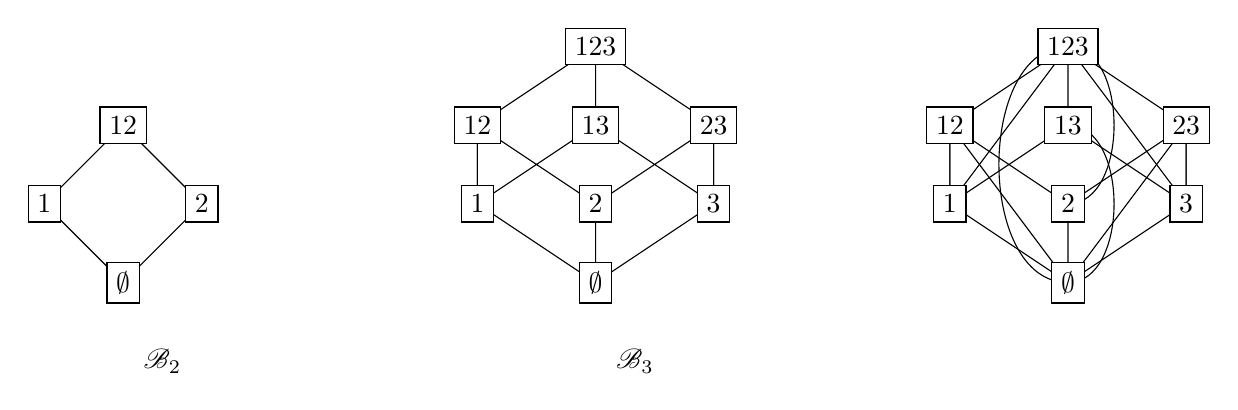
\begin{tikzpicture}
\newcommand{\hshft}{6}
\draw (1,0) -- (0,1) -- (1,2) -- (2,1) -- cycle;
\node[draw, fill=white] at (1,0) {$\0$};
\node[draw, fill=white] at (0,1) {$1$};
\node[draw, fill=white] at (2,1) {$2$};
\node[draw, fill=white] at (1,2) {$12$};
\node at (1.5,-1){$\BB_2$};
\begin{scope}[shift={(\hshft,0)}]
\draw (1,3) -- (-.5,2) -- (-.5,1) -- (1,0) -- (2.5,1) -- (2.5,2) -- (1,3) -- (1,2);
\draw (1,0) -- (1,1) -- (2.5,2) -- (2.5,1) -- (1,2) -- (-.5,1) -- (-.5,2) -- (1,1);
\node[draw, fill=white] at (1,0) {$\0$};
\node[draw, fill=white] at (-.5,1) {$1$};
\node[draw, fill=white] at (1,1) {$2$};
\node[draw, fill=white] at (2.5,1) {$3$};
\node[draw, fill=white] at (-.5,2) {$12$};
\node[draw, fill=white] at (1,2) {$13$};
\node[draw, fill=white] at (2.5,2) {$23$};
\node[draw, fill=white] at (1,3) {$123$};
\node at (1.5,-1){$\BB_3$};
\end{scope}
\begin{scope}[shift={(2*\hshft,0)}]
\draw (1,3) -- (-.5,2) -- (-.5,1) -- (1,0) -- (2.5,1) -- (2.5,2) -- (1,3) -- (1,2);
\draw (1,0) -- (1,1) -- (2.5,2) -- (2.5,1) -- (1,2) -- (-.5,1) -- (-.5,2) -- (1,1);
\draw (-.5,2) -- (1,0) -- (2.5,2);
\draw (-.5,1) -- (1,3) -- (2.5,1);
\draw (1,0) to [out = 180, in = 180] (1,3);
\draw (1,0) to [out = 0, in = 0] (1,2);
\draw (1,1) to [out = 0, in = 0] (1,3);
\node[draw, fill=white] at (1,0) {$\0$};
\node[draw, fill=white] at (-.5,1) {$1$};
\node[draw, fill=white] at (1,1) {$2$};
\node[draw, fill=white] at (2.5,1) {$3$};
\node[draw, fill=white] at (-.5,2) {$12$};
\node[draw, fill=white] at (1,2) {$13$};
\node[draw, fill=white] at (2.5,2) {$23$};
\node[draw, fill=white] at (1,3) {$123$};
\end{scope}
\end{tikzpicture}
\end{center}
Note that $2^{[n]}$ is a lattice, with meet and join given by intersection and union respectively.
\end{example}

The first two pictures are \defterm{Hasse diagrams}: graphs whose vertices are the elements of the poset
and whose edges represent the \defterm{covering relations}, which are enough to generate all the relations
in the poset by transitivity.  (As you can see on the right, including \emph{all} the relations would
make the diagram unnecessarily complicated.)  By convention, bigger elements in $P$ are at the top of the picture.

The Boolean algebra $2^S$ has a unique minimum element (namely $\emptyset$) and a
unique maximum element (namely $S$).  Not every poset has to have such elements,
but if a poset does, we will call them $\hatzero$ and $\hatone$ respectively
(or if necessary $\hatzero_P$ and $\hatone_P$).

\begin{definition}  A poset that has both a $\hatzero$ and a $\hatone$ is called \defterm{bounded}.\footnote{This has nothing to do with the more typical metric-space definition of ``bounded''.}  An element that covers $\hatzero$ is called an \defterm{atom}, and an element that is covered by $\hatone$ is called a \defterm{coatom}.  For example, the atoms in $2^S$ are the singleton subsets of $S$, and the coatoms are the subsets of cardinality $|S|-1$.
\end{definition}

We can make a poset $P$ bounded: define a new poset $\hat P$ by adjoining new elements $\hatzero,\hatone$ such that $\hatzero<x<\hatone$ for every $x\in P$.  Meanwhile, sometimes we have a bounded poset and want to delete the bottom and top elements.

\begin{definition}
The \defterm{interval} from $x$ to $y$ is
\[[x,y]:=\{z\in P\st x\leq z\leq y\}.\]
This is nonempty if and only if $x\leq y$, and it is a singleton set if and only if $x=y$.%  For example, every nonempty interval $[A,B]\subseteq 2^{[n]}$ is itself a Boolean algebra of rank $|B|-|A|$.  (The proof is an exercise.)
\end{definition}

\begin{definition} A subset $C\subseteq P$ (or $P$ itself) is called a \defterm{chain} if its elements are pairwise comparable.
Thus every chain is of the form $C=\{x_0,\dots,x_n\}$, where $x_0<\cdots<x_n$.
An \defterm{antichain} is a subset of $P$ (or, again, $P$ itself) in which no two of its elements are comparable.\footnote{To set theorists, ``antichain'' means something stronger: a set of elements such that no two have a common lower bound.  This concept does not typically arise in combinatorics, where one frequently wants to talk about antichains in a bounded posets.}
\end{definition}

\begin{center}
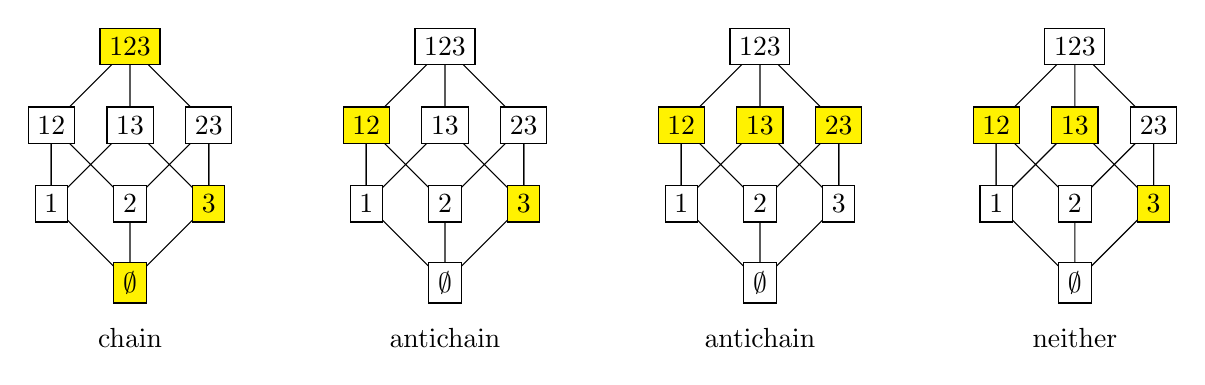
\begin{tikzpicture}
\newcommand{\hshft}{4}
\draw (1,3) -- (0,2) -- (0,1) -- (1,0) -- (2,1) -- (2,2) -- (1,3) -- (1,2);
\draw (1,0) -- (1,1) -- (2,2) -- (2,1) -- (1,2) -- (0,1) -- (0,2) -- (1,1);
\node[draw, fill=yellow] at (1,0) {$\0$};
\node[draw, fill=white] at (0,1) {$1$};
\node[draw, fill=white] at (1,1) {$2$};
\node[draw, fill=yellow] at (2,1) {$3$};
\node[draw, fill=white] at (0,2) {$12$};
\node[draw, fill=white] at (1,2) {$13$};
\node[draw, fill=white] at (2,2) {$23$};
\node[draw, fill=yellow] at (1,3) {$123$};
\node at (1,-.7) {chain};

\begin{scope}[shift={(\hshft,0)}]
\draw (1,3) -- (0,2) -- (0,1) -- (1,0) -- (2,1) -- (2,2) -- (1,3) -- (1,2);
\draw (1,0) -- (1,1) -- (2,2) -- (2,1) -- (1,2) -- (0,1) -- (0,2) -- (1,1);
\node[draw, fill=white] at (1,0) {$\0$};
\node[draw, fill=white] at (0,1) {$1$};
\node[draw, fill=white] at (1,1) {$2$};
\node[draw, fill=yellow] at (2,1) {$3$};
\node[draw, fill=yellow] at (0,2) {$12$};
\node[draw, fill=white] at (1,2) {$13$};
\node[draw, fill=white] at (2,2) {$23$};
\node[draw, fill=white] at (1,3) {$123$};
\node at (1,-.7) {antichain};
\end{scope}
\begin{scope}[shift={(2*\hshft,0)}]
\draw (1,3) -- (0,2) -- (0,1) -- (1,0) -- (2,1) -- (2,2) -- (1,3) -- (1,2);
\draw (1,0) -- (1,1) -- (2,2) -- (2,1) -- (1,2) -- (0,1) -- (0,2) -- (1,1);
\node[draw, fill=white] at (1,0) {$\0$};
\node[draw, fill=white] at (0,1) {$1$};
\node[draw, fill=white] at (1,1) {$2$};
\node[draw, fill=white] at (2,1) {$3$};
\node[draw, fill=yellow] at (0,2) {$12$};
\node[draw, fill=yellow] at (1,2) {$13$};
\node[draw, fill=yellow] at (2,2) {$23$};
\node[draw, fill=white] at (1,3) {$123$};
\node at (1,-.7) {antichain};
\end{scope}
\begin{scope}[shift={(3*\hshft,0)}]
\draw (1,3) -- (0,2) -- (0,1) -- (1,0) -- (2,1) -- (2,2) -- (1,3) -- (1,2);
\draw (1,0) -- (1,1) -- (2,2) -- (2,1) -- (1,2) -- (0,1) -- (0,2) -- (1,1);
\node[draw, fill=white] at (1,0) {$\0$};
\node[draw, fill=white] at (0,1) {$1$};
\node[draw, fill=white] at (1,1) {$2$};
\node[draw, fill=yellow] at (2,1) {$3$};
\node[draw, fill=yellow] at (0,2) {$12$};
\node[draw, fill=yellow] at (1,2) {$13$};
\node[draw, fill=white] at (2,2) {$23$};
\node[draw, fill=white] at (1,3) {$123$};
\node at (1,-.7) {neither};
\end{scope}
\end{tikzpicture}
\end{center}

\begin{definition}
A \defterm{linear extension} of a poset $P$ is a total order $\prec$ on the set $P$ that refines $<_P$: that is, if $x<_Py$ then $x\prec y$.  The set of all linear extensions is denoted $\LL(P)$ (and sometimes called the \emph{Jordan-H\"{o}lder set of $P$}).
\end{definition}

If $P$ is a chain then $\LL(P)=\{P\}$, while if $P$ is an antichain then $\LL(P)=\Sym_P$.  In general, the more relations $P$ has, the fewer linear extensions. % If $P$ and $Q$ are chains, then $\LL(P+Q)$ is the set of \defterm{shuffles} of $P\dju Q$: linear orderings in which the ordering of each summand is preserved.  In this case $|\LL(P+Q)|=\binom{|P|+|Q|}{|P|}$.

\begin{definition}
A \defterm{subposet} of $P$ is a subset  $Q\subseteq P$ that shares the same order relation, i.e., for $q,q'\in Q$, we have $q\leq_Qq'$ if and only if $q\leq_Pq'$.
\end{definition}

\begin{definition} \label{def:order-ideal}
An \defterm{order ideal} (resp., an \defterm{order filter}) of $P$ is a subposet $Q\subseteq P$ with the property that if $x,y\in P$, $x\in Q$, and $y\leq x$ (resp., $y\geq x$) then $y\in Q$.
\end{definition}

Colloquially, an order ideal is a subset of $P$ ``closed under going down''.  Note that a subset of $P$ is an order ideal if and only if its complement is an order filter.  The order ideal \defterm{generated} by $Q\subseteq P$ is the smallest order ideal containing it, namely $\langle Q\rangle=\{x\in P \st x\leq q\text{ for some } q\in Q\}$.  Conversely, every order ideal has a unique minimal set of generators, namely its maximal elements (which form an antichain).

\begin{example}
Let $\{F_1,\dots,F_k\}$ be a nonempty family of subsets of $[n]$.  The order ideal they generate is
\[\Delta=\langle F_1,\dots, F_k\rangle = \left\{G\subseteq[n] \st G\subseteq F_i \text{ for some }i\right\}.\]
These order ideals are called \defterm{abstract simplicial complexes}, and are the standard combinatorial models for topological spaces (at least well-behaved ones).  If each $F_i$ is regarded as a simplex (i.e., the convex hull of a set of affinely independent points) then the order-ideal condition says that if $\Delta$ contains a simplex, then it contains all sub-simplices.  For example, $\Delta$ cannot contain a triangle without also containing its edges and vertices.  We will have much, much more to say about simplicial complexes in Section~\ref{sec:simplicial}.
\end{example}

%------------------------------------------------------------
\subsection{Operations on posets}

\begin{definition}
Let $P,Q$ be posets.
\begin{itemize}
\item
The \defterm{dual} $P^*$ of $P$ is obtained by reversing all the order relations: $x\leq_{P^*}y$ iff $x\geq_Py$.  The Hasse diagram of $P^*$ is the same as that of~$P$, turned upside down.  A poset is \defterm{self-dual} if $P\isom P^*$; the map realizing the self-duality is called an \defterm{anti-automorphism}.  For example, chains and antichains are self-dual, as is $\BB_n$ (via the anti-automorphism $S\mapsto[n]\sm S$).
\item
The \defterm{disjoint union} $P+Q$ is the poset on $P\dju Q$ that inherits the relations from $P$ and $Q$ but no others, so that elements of $P$ are incomparable with elements of~$Q$.  The Hasse diagram of $P+Q$ can be obtained by drawing the Hasse diagrams of $P$ and $Q$ side by side.
\item
The \defterm{Cartesian product} $P\x Q$ has a poset structure as follows: $(p,q)\leq(p',q')$ if $p\leq_Pp'$ and $q\leq_Qq'$.
This is a very natural and useful operation.  For example, it is not hard to check that $\BB_k\x\BB_{\ell}\isom\BB_{k+\ell}$.
\item
Assume that $P$ has a $\hatone$ and $Q$ has a $\hatzero$.  Then the \defterm{ordinal sum} $P\oplus Q$ is defined by identifying $\hatone_P=\hatzero_Q$ and setting $p\leq q$ for all $p\in P$ and $q\in Q$.
\end{itemize}
\end{definition}

\begin{figure}[ht]
\begin{center}
\begin{tikzpicture}
% P
\node at (0,-2) {\Large$P$};
\foreach \p in {(0,0),(0,-1),(.7,.7),(-.7,.7),(0,1.4)}  \draw[fill=black] \p circle(.6ex);
\draw (0,0) -- (.7,.7) -- (0,1.4) -- (-.7,.7) -- (0,0) -- (0,-1);
% Q
\begin{scope}[shift={(3,0)}]
    \foreach \p in {(0,0),(.7,.7),(-.7,.7)} \draw[red, fill=red] \p circle(.6ex);
    \draw[red] (-.7,.7) -- (0,0) -- (.7,.7);
    \node at (0,-2) {\Large\Red{$Q$}};
\end{scope}
% Direct product
\begin{scope}[shift={(6,1)}]
    \foreach \p in {(0,0),(0,-1),(.7,.7),(-.7,.7),(0,1.4)}
    {
        \begin{scope}[shift={\p}]
            \draw[red] (0,0) -- (2,-1) -- (4,0);
        \end{scope}
        \draw[fill=black] \p circle(.6ex);
    }
    \draw (0,0) -- (.7,.7) -- (0,1.4) -- (-.7,.7) -- (0,0) -- (0,-1);
    \begin{scope}[shift={(2,-1)}]
        \foreach \p in {(0,0),(0,-1),(.7,.7),(-.7,.7),(0,1.4)}  \draw[fill=black] \p circle(.6ex);
        \draw (0,0) -- (.7,.7) -- (0,1.4) -- (-.7,.7) -- (0,0) -- (0,-1);
        \node at (0,-2) {\Large$P\x Q$};
    \end{scope}
    \begin{scope}[shift={(4,0)}]
        \foreach \p in {(0,0),(0,-1),(.7,.7),(-.7,.7),(0,1.4)}  \draw[fill=black] \p circle(.6ex);
        \draw (0,0) -- (.7,.7) -- (0,1.4) -- (-.7,.7) -- (0,0) -- (0,-1);
    \end{scope}
\end{scope}
% Ordinal sum
\begin{scope}[shift={(13,0)}]
    \foreach \p in {(0,0),(0,-1),(.7,.7),(-.7,.7),(0,1.4)}  \draw[fill=black] \p circle(.6ex);
    \draw (0,0) -- (.7,.7) -- (0,1.4) -- (-.7,.7) -- (0,0) -- (0,-1);
    \begin{scope}[shift={(0,1.4)}]
        \foreach \p in {(0,0),(.7,.7),(-.7,.7)} \draw[red, fill=red] \p circle(.6ex);
        \draw[red] (-.7,.7) -- (0,0) -- (.7,.7);
    \end{scope}
    \node at (0,-2) {\Large$P\oplus Q$};
\end{scope}
\end{tikzpicture}
\end{center}
\caption{Direct product $\x$ and ordinal sum $\oplus$. \label{fig:poset-ops}}
\end{figure}


%------------------------------------------------------------
\subsection{Ranked posets}

One of the many nice properties of the Boolean algebra $\BB_n$ is that its elements fall nicely into horizontal slices (sorted by their cardinalities).  Whenever $S\coveredby T$, it is the case that $|T|=|S|+1$.  A poset for which we can do this is called a \defterm{ranked} poset.  However, it would be tautological to define a ranked poset to be a poset in which we can rank the elements.  The actual definition of rankedness is a little more subtle, but makes perfect sense after a little thought.

\begin{definition} \label{saturated-ranked}
A chain $x_0<\cdots<x_n$ is \defterm{saturated}\footnote{%
Sometimes called ``maximal'', but that word can easily be misinterpreted to mean ``of maximum size''.}
if it is not properly contained in any other chain from~$x_0$ to~$x_n$; equivalently, if $x_{i-1}\coveredby x_i$ for every $i\in[n]$.  In this case, the number $n$ is the \defterm{length} of the chain.
A poset $P$ is \defterm{ranked} if for every $x\in P$, all saturated chains with top element~$x$ have the same length; this number is called the \defterm{rank} of $x$ and denoted $r(x)$.  It follows that
\begin{equation} \label{rank-increment}
x\coveredby y ~\implies~ r(y)=r(x)+1.
\end{equation}
A poset is \defterm{graded} if it is ranked and bounded.
\end{definition}

\begin{note}
\begin{enumerate}
\item ``Length'' means the number of \emph{steps}, not the number
of \emph{elements} --- i.e., edges rather than vertices in the
Hasse diagram.
\item The literature is not
consistent on the usage of the term ``ranked''. Sometimes ``ranked'' is 
used for the weaker condition that for every pair $x,y\in P$, every 
chain from $x$ to $y$ has the same length.  Under this definition,
the implication \eqref{rank-increment} fails (proof left to the reader).
\item For any finite poset $P$ (and some infinite ones) one can define $r(x)$ to be the supremum
of the lengths of all chains with top element $x$ --- but if $P$ is not a ranked poset,
then there will be some pair $x,y$ such that $y\covers x$ but $r(y)>r(x)+1$.
For instance, in the bounded poset shown below (known as $N_5$), we have $\hatone\covers y$,
but $r(\hatone)=3$ and $r(y)=1$.
\end{enumerate}
\end{note}
\[\xymatrix@R=0.6pc{
&\hatone\linedl\lineddr\\
z\linedd\\
&&y\lineddl\\
x\linedr\\
&\hatzero
}\]

\begin{definition} Let $P$ be a ranked poset with rank function $r$.
The \defterm{rank-generating function} of $P$ is the formal power series
\[F_P(q) = \sum_{x\in P} q^{r(x)}.\]
Thus, for each~$k$, the coefficient of $q^k$ is the number of elements at rank~$k$.
\end{definition}

For example, the Boolean algebra is ranked by cardinality, with
\[F_{\BB_n}(q) = \sum_{S\subseteq[n]} q^{|S|} = (1+q)^n.\]
The expansion of this polynomial is palindromic, because the 
coefficients are a row of Pascal's Triangle.  That is, $\BB_n$ is 
\defterm{rank-symmetric}.  Rank-symmetry also follows from the self-duality of $\BB_n$.

More generally, if $P$ and $Q$ are ranked, then $P\x Q$ is ranked, with $r_{P|x Q}(x,y)=r_P(x)+r_Q(y)$, and $F_{P\x Q}=F_PF_Q$.

\subsection{Lattices}

\begin{definition} A poset $L$ is a \defterm{lattice} if every pair $x,y\in L$ has a unique \defterm{meet} $x\meet y$ and \defterm{join} $x\join y$.  That is,
\begin{align*}
x\meet y &= \max\{z\in L ~|~ z\leq x \text{ and } z\leq y\},\\
x\join y &= \min\{z\in L ~|~ z\geq x \text{ and } z\geq y\}.
\end{align*}
\end{definition}

Note that, e.g., $x\meet y=x$ if and only if $x\leq y$.  Meet and join are easily seen to be commutative and associative, so for any finite $M\subseteq L$, the meet $\meet M$ and join $\join M$ are well-defined elements of $L$.  In particular, every finite lattice is bounded, with $\hatzero=\meet L$ and $\hatone=\join L$.  For convenience, we set $\meet\0=\hatone$ and $\join\0=\hatzero$.

\begin{example}[\textbf{The partition lattice}]
Let $\Pi_n$ be the poset of all
set partitions of $[n]$.  E.g., two elements of $\Pi_5$ are
\[
\begin{array}{ll}
\pi = \big\{\{1,3,4\},\ \{2,5\}\big\} & \qquad\text{(abbr.: } 134|25)\\
\sigma = \big\{\{1,3\},\ \{4\},\ \{2,5\}\big\} & \qquad\text{(abbr.: } 13|4|25)
\end{array}
\]
The sets $\{1,3,4\}$ and $\{2,5\}$ are called the \defterm{blocks} of $\pi$.
We can impose a partial order on $\Pi_n$ by putting $\sigma\leq \pi$ if every
block of $\sigma$ is contained in a block of $\pi$; for short, $\sigma$ \defterm{refines}
$\pi$.

\[\xymatrix@C=0.8pc{
&&&&&&&& 1234\linedlll\linedll\linedl\lined\linedr\linedrr\linedrrr\\
 & 123 \linedl\lined\linedr      &&&&      123|4\lined\linedr\linedrr & 124|3\linedl\linedrr\linedrrr & 134|2\linedl\linedr\linedrrr & 234|1\linedl\linedr\linedrr & 12|34\linedllll\linedr & 13|24\linedllll\linedl & 14|23\linedllll\linedlll\\
12|3 & 1|23 & 13|2      &&&      12|3|4 & 13|2|4 & 23|1|4 & 14|2|3 & 24|1|3 & 34|1|2\\
 & 1|2|3 \lineul\lineu\lineur      && \text{\boldmath\Large$\Pi_3$} &&&&&      1|2|3|4 \lineulll\lineull\lineul\lineu\lineur\lineurr && \text{\boldmath\Large$\Pi_4$}
}  \]

Observe that $\Pi_n$ is bounded, with $\hatzero=1|2|\cdots|n$ and $\hatone=12\cdots n$.
For each partition $\sigma$, the partitions that cover $\sigma$ in~$\Pi_n$ are those obtained from $\sigma$ by merging two of its blocks into a single block.  Therefore, $\Pi_n$ is ranked (hence graded), with rank function $r(\pi)=n-|\pi|$.
The coefficients of the rank-generating function of $\Pi_n$ are by definition the Stirling numbers of the second kind.  Recall that $S(n,k)$ is the number of partitions of $[n]$ into $k$ blocks, so
\[F_{\Pi_n}(q) = \sum_{k=1}^n S(n,k)q^{n-k}.\]

Furthermore, $\Pi_n$ is a lattice.  The meet of two partitions is their coarsest common refinement: $x,y$ belong to the 
same block of $\pi\meet \sigma$ if and only if they belong to the same block of $\pi$ and to the same block of $\sigma$.
The join is the transitive closure of the union of the equivalence relations corresponding to $\pi$ and $\sigma$.

Finally, for any finite set, we can define $\Pi_X$ to be the poset of set partitions of $X$, ordered by reverse refinement; evidently $\Pi_X\isom\Pi_{|X|}$.
\end{example}

\begin{example}[\textbf{The connectivity lattice of a graph}]\label{KG}
Let $G=(V,E)$ be a (simple) graph.  Recall that for $X\subseteq V$, the \emph{induced subgraph} $G|_X$ is the graph on vertex set $X$, with two edges adjacent in $G|_X$ if and only iff they are adjacent in~$G$.
The \defterm{connectivity lattice} of $G$ is the subposet of $\Pi_V$ defined by
\[K(G) = \{\pi\in\Pi_V \st G|_X\text{ is connected for every block } X\in\pi\}.\]
For an example, see Figure~\ref{fig:KG}.
It is not hard to see that $K(G)=\Pi_V$ if and only if $G$ is the complete graph $K_V$, and $K(G)$ is Boolean if and only if $G$ is acyclic.  Also, if $H$ is a subgraph of $G$ then $K(H)$ is a subposet of $K(G)$.  The proof that $K(G)$ is in fact a lattice (justifying the terminology) is left as an exercise.

\begin{figure}[ht]
\begin{center}
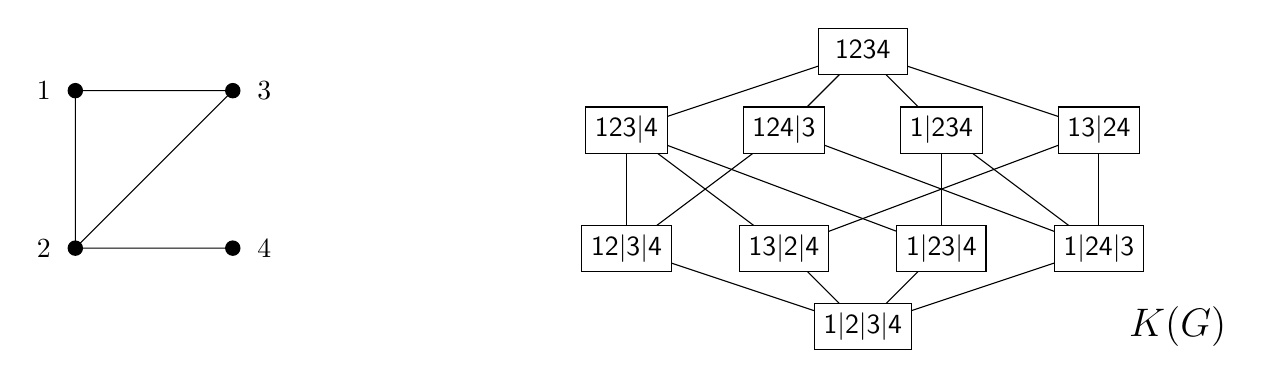
\begin{tikzpicture}
\foreach \x in {0,2} \foreach \y in {0,2} \draw[fill=black] (\x,\y) circle(.6ex);
\draw (0,0) -- (2,2) -- (0,2) -- (0,0) -- (2,0);
\node at (-.4,2) {1};
\node at (-.4,0) {2};
\node at (2.4,2) {3};
\node at (2.4,0) {4};

\begin{scope}[shift={(10,0)}]
\foreach \x in {-3,-1,1,3}
{
    \draw (0,-1) -- (\x,0);
    \draw (0,2.5) -- (\x,1.5);
}
\foreach \x in {-3,-1} \draw (-3,0) -- (\x,1.5);
\foreach \x in {-3,3} \draw (-1,0) -- (\x,1.5);
\foreach \x in {-3,1} \draw (1,0) -- (\x,1.5);
\foreach \x in {-1,1,3} \draw (3,0) -- (\x,1.5);
\node[draw, fill=white] at (0,-1) {$\mathsf{1|2|3|4}$};
\node[draw, fill=white] at (-3,0) {$\mathsf{12|3|4}$};
\node[draw, fill=white] at (-1,0) {$\mathsf{13|2|4}$};
\node[draw, fill=white] at (1,0) {$\mathsf{1|23|4}$};
\node[draw, fill=white] at (3,0) {$\mathsf{1|24|3}$};
\node[draw, fill=white] at (-3,1.5) {$\mathsf{123|4}$};
\node[draw, fill=white] at (-1,1.5) {$\mathsf{124|3}$};
\node[draw, fill=white] at (1,1.5) {$\mathsf{1|234}$};
\node[draw, fill=white] at (3,1.5) {$\mathsf{13|24}$};
\node[draw, fill=white] at (0,2.5) {$\phantom{|}\mathsf{1234}\phantom{|}$};
\node at (4,-1) {\Large $K(G)$};
\end{scope}
\end{tikzpicture}
\end{center}
\caption{A graph and its connectivity lattice.\label{fig:KG}}
\end{figure}
\end{example}

\begin{example}[\textbf{Young's lattice}]
An \defterm{(integer) partition} is a sequence
$\lambda=(\lambda_1,\dots,\lambda_\ell)$ of weakly decreasing positive
integers: i.e., $\lambda_1\geq\cdots\geq\lambda_\ell>0$.  If $n=\lambda_1+\cdots+\lambda_\ell$, we write $\lambda\partn n$ and/or $n=|\lambda|$.
For convenience,
set $\lambda_i=0$ for all $i>\ell$.  Let $Y$ be the set of all partitions,
partially ordered by $\lambda\geq\mu$
if $\lambda_i\geq\mu_i$ for all $i=1,2,\dots$.
Then $Y$ is a ranked lattice, with rank function $r(\lambda)=|\lambda|$.  Join and meet are given by component-wise max and min --- we'll shortly see another description of the lattice operations.
\end{example}

This is an infinite poset, but the number of  partitions at any given rank is finite.
So in particular $Y$ is \defterm{locally finite} (if $X$ is any adjective, then ``poset $P$ is locally $X$'' means ``every interval in $P$ is $X$'').  Moreover, the rank-generating function
\[ \sum_{\lambda} q^{|\lambda|} = \sum_{n\geq0} \sum_{\lambda\partn n} q^n \]
is a well-defined formal power series, and it is given by the justly celebrated formula
\[ \prod_{k=1}^\infty \frac{1}{1-q^k}.\]

There is a nice pictorial way to look at Young's lattice.  Instead of thinking
about partitions as sequence of numbers, view them as their corresponding
\defterm{Ferrers diagrams} (or \defterm{Young diagrams}): northwest-justified piles of boxes whose
$i^{th}$ row contains $\lambda_i$ boxes.  The northwest-justification convention is called ``English notation'', and I will use that throughout, but a significant minority of combinatorialists prefer ``French notation'', in which the vertical axis is reversed.  For example, the partition $(5,5,4,2)$ is represented by the Ferrers diagram
\ytableausetup{smalltableaux}
\[\raisebox{0.65cm}{\ydiagram{5,5,4,2}} \quad \textrm{(English)} \qquad \qquad \text{or} \qquad \qquad
\reflectbox{\rotatebox{180}{\ydiagram{5,5,4,2}}} \quad \textrm{(French).}
\]

Now the order relation in Young's lattice is as follows: $\lambda\geq\mu$ if and only the Ferrers diagram of $\lambda$ contains
that of $\mu$.  The bottom part of the Hasse diagram of~$Y$ looks like this:

\includefigure{3in}{2in}{young}

In terms of Ferrers diagrams, join and meet are simply union and intersection respectively.

Young's lattice $Y$ has a nontrivial automorphism $\lambda\mapsto\tilde\lambda$
called \defterm{conjugation}.
This is most easily described in terms of Ferrers diagrams: reflect across the line
$x+y=0$ so as to swap rows and columns.  It is easy to check that if $\lambda\geq\mu$, then
$\tilde\lambda\geq\tilde\mu$.

\begin{example}[\textbf{The subspace lattice}]
Let $q$ be a prime power, let $\Ff_q$ be the field of order~$q$,
and let $V=\Ff_q^n$ (a vector space of dimension~$n$ over $\Ff_q$).  The \emph{subspace lattice}
$L_V(q)=L_n(q)$ is the set of all vector subspaces of $V$, ordered by inclusion.  (We could replace
$\Ff_q$ with any old field if you don't mind infinite posets.)

The meet and join operations on $L_n(q)$ are given by $W\meet W'=W\cap W'$
and $W\join W'=W+W'$.  We could construct analogous posets by
ordering the (normal) subgroups of a group, or the prime ideals of a ring, or the
submodules of a module, by inclusion.  (However, these posets are not necessarily
ranked, while $L_n(q)$ is ranked, by dimension.)

The simplest example is when $q=2$ and $n=2$, so that $V=\{(0,0),(0,1),(1,0),(1,1)\}$.
Of course $V$ has one subspace of dimension~2 (itself) and one of dimension~0 (the zero space).
Meanwhile, it has three subspaces of dimension~1; each consists of the zero vector and
one nonzero vector.  Therefore, $L_2(2)\isom M_5$.
\begin{center}
\begin{tikzpicture}[scale=\tikzposetscale]
\draw (0,0) -- (-1.5,1.5) -- (0,3) -- (1.5,1.5) -- (0,0) -- (0,3);
\foreach \v in {(0,0),(-1.5,1.5),(0,1.5),(1.5,1.5),(0,3)} \draw[fill=black] \v circle (\tikzvertexsize);
\node at (1.5,-.5) {$M_5$};
%\node at (-2,1.5) {$a$};
%\node at (-.5,1.5) {$b$};
%\node at (2,1.5) {$c$};
\end{tikzpicture}
\end{center}
Note that $L_n(q)$ is self-dual, under the anti-automorphism $W\to W^\perp$ (the orthogonal complement with respect to any non-degenerate bilinear form).
\end{example}

\begin{example}
Lattices don't have to be ranked.  For example, the poset $N_5$ shown below is a
perfectly good lattice.
\begin{center}
\begin{tikzpicture}[scale=\tikzposetscale]
\draw (0,0) -- (1.5,1.5) -- (0,3) -- (-1,2.1) -- (-1,.9) -- (0,0);
\foreach \v in {(0,0),(1.5,1.5),(0,3),(-1,2.1),(-1,.9)} \draw[fill=black] \v circle (\tikzvertexsize);
\node at (1,-.5) {$N_5$};
%\node at (-1.6,.9) {$x$};
%\node at (-1.6,2.1) {$z$};
%\node at (2.1,1.5) {$y$};
\end{tikzpicture}
\end{center}
\end{example}

\begin{proposition}[\textbf{Absorption laws}]
Let $L$ be a lattice and $x,y\in L$.  Then $x\join(x\meet y)=x$
and $x\meet(x\join y)=x$. (Proof left to the reader.)
\end{proposition}

The following result is a very common way of proving that a poset is a lattice.

\begin{proposition} \label{bounded-semilattice}
Let $P$ be a bounded poset that is a meet-semilattice (i.e., every nonempty $B\subseteq P$ has a well-defined meet $\meet B$).  Then every finite nonempty subset of $P$ has a well-defined join, and consequently $P$ is a lattice.  Similarly, every bounded join-semilattice is a lattice.
\end{proposition}
\begin{proof}
Let $P$ be a bounded meet-semilattice.
Let $A\subseteq P$, and let $B=\{b\in P\st b\geq a$ for all $a\in A\}$.
Note that $B\neq\emptyset$ because $\hatone\in B$.
I claim that $\meet B$ is the unique least upper bound for $A$.
First, we have $\meet B\geq a$ for all $a\in A$ by definition of $B$ and of meet.
Second, if $x\geq a$ for all $a\in A$, then $x\in B$ and so $x\geq\meet B$,
proving the claim.  The proof of the second assertion is dual to this proof.
\end{proof}

\begin{definition}
Let $L$ be a lattice.  A \defterm{sublattice} of $L$ is a subposet $L'\subseteq L$
that (a) is a lattice and (b) inherits its meet and join operations from $L$.
That is, for all $x,y\in L'$, we have
\[x\meet_{L'} y = x\meet_L y \qandq x\join_{L'} y = x\join_L y.\]
\end{definition}

The maximum and minimum elements of a sublattice of $L$ need not be the same as those of $L$.
As an important example, every interval $L'=[x,z]\subseteq L$ (i.e., $L'=\{y\in L\st x\leq y\leq z\}$)
is a sublattice with minimum element $x$ and maximum element $z$.  (We might write $\hatzero_{L'}=x$
and $\hatone_{L'}=z$.)

\begin{example}
Young's lattice $Y$ is an infinite lattice.  Meets of arbitrary sets are well-defined, as are finite joins.  There is an $\hatzero$ element (the empty Ferrers diagram), but no $\hatone$.  On the other hand, $Y$ is \defterm{locally finite} --- every interval $[\lambda,\mu]\subseteq Y$ is finite.  Similarly, the set of natural numbers, partially ordered by divisibility, is an infinite, locally finite lattice with a $\hat0$ element.
\end{example}

\begin{example}\label{ex:Bruhat}[\textbf{Weak Bruhat order}]
Let $\Sym_n$ be the set of permutations of 
$[n]$ (i.e., the symmetric group).\footnote{That's a Fraktur S, obtainable in LaTeX as {\tt $\backslash$mathfrak$\{$S$\}$}.  The letter $S$ has many other standard uses in combinatorics:
Stirling numbers of the first and second kind, Schur symmetric functions, etc.  The symmetric group is
important enough to merit an ornate symbol!} Write elements $w\in\Sym_n$ as strings
$w_1w_2\cdots w_n$ of distinct digits, e.g., $47182635\in\Sym_8$.  (This is called \emph{one-line notation}.)
The \defterm{weak Bruhat order} on $\Sym_n$ is defined as follows:
$w\coveredby v$ if $v$ can be obtained by swapping $w_i$
with $w_{i+1}$, where $w_i<w_{i+1}$.  For example,
\[4716\underline{\bf28}35 \coveredby 4716\underline{\bf82}35 \qandq 4\underline{\bf71}62835 \covers 4\underline{\bf17}62835.\]
In other words, $s_i<w_{i+1}$ and $v=w s_i$, where $s_i$ is the transposition that swaps $i$ with $i+1$.
The weak order actually is a lattice, though this is not so easy to prove.

The \defterm{Bruhat order} on permutations is a related partial order with more relations (i.e., ``stronger'') than the weak order.  We first need the notion of \defterm{inversions}: an inversion of $w\in\Sym_n$ is an ordered pair $(i,j)$ such that $i<j$ and $w_i>w_j$.  The number of inversions is written $\inv(w)$.  The simplest way of describing Bruhat order is as follows: $w\coveredby v$ if $\inv(v)=\inv(w)+1$ and $v=wt$ for some transposition~$t$.  For example, 
\[471\underline{\bf6}2\underline{\bf8}35 \coveredby 471\underline{\bf8}2\underline{\bf6}35\]
in Bruhat order (because this transposition has introduced exactly one more inversion), but not in weak order (since the positions transposed, namely 4 and 6, are not adjacent).  On the other hand,
$47\underline{\bf1}62\underline{\bf8}35$ is not covered by $47\underline{\bf8}62\underline{\bf1}35$ because this transposition increases the inversion number by~3, not by~1.

The Bruhat and weak orders on $\Sym_3$ are shown below.  You should be able to see from the picture that Bruhat order is not a lattice.
\begin{center}
\begin{tikzpicture}[scale=\tikzposetscale]
\draw (0,0) -- (-1.5,1) -- (-1.5,3) -- (0,4) -- (1.5,3) -- (1.5,1) -- cycle;
\draw (-1.5,1) -- (1.5,3);
\draw (1.5,1) -- (-1.5,3);
\foreach \v in {(0,0),(-1.5,1),(-1.5,3),(0,4),(1.5,3),(1.5,1)} \draw[fill=black] \v circle (\tikzvertexsize);
\node at (0,-.5) {123};
\node at (-2.25,1) {132};
\node at (2.25,1) {213};
\node at (-2.25,3) {312};
\node at (2.25,3) {231};
\node at (0,4.5) {321};
\node at (0,-1.5) {Bruhat order};
\begin{scope}[shift={(12,0)}]
\draw (0,0) -- (-1.5,1) -- (-1.5,3) -- (0,4) -- (1.5,3) -- (1.5,1) -- cycle;
\foreach \v in {(0,0),(-1.5,1),(-1.5,3),(0,4),(1.5,3),(1.5,1)} \draw[fill=black] \v circle (\tikzvertexsize);
\node at (0,-.5) {123};
\node at (-2.25,1) {132};
\node at (2.25,1) {213};
\node at (-2.25,3) {312};
\node at (2.25,3) {231};
\node at (0,4.5) {321};
\node at (0,-1.5) {Weak Bruhat order};
\end{scope}
\end{tikzpicture}
\end{center}

A \emph{Coxeter group} is a finite group generated by elements
$s_1,\dots,s_n$, called \emph{simple reflections}, satisfying
$s_i^2=1$ and $(s_is_j)^{m_{ij}}=1$ for all $i\neq j$ and some
integers $m_{ij}\geq23$.  For example, setting $m_{ij}=3$ if
$|i-j|=1$ and $m_{ij}=2$ if $|i-j|>1$, we obtain the symmetric group
$\Sym_{n+1}$.  Coxeter groups are fantastically important in geometric
combinatorics and we could spend at least a semester on them.  The standard resources are the books by Brenti and Bj\"orner~\cite{BB}, which has a more combinatorial approach, and Humphreys~\cite{Humphreys}, which has a more geometric flavor.  For
now, it's enough to mention that every Coxeter group has associated
Bruhat and weak orders, whose definitions generalize those for the symmetric group.

The Bruhat and weak order give graded, self-dual poset structures on
$\Sym_n$, with the same rank function, namely the number
of \defterm{inversions}:
\[r(w) = \Big|\big\{\{i,j\} \st i<j~\text{and}~w_i>w_j\big\}\Big|.\]
(For a general Coxeter group, the rank of an element $w$ is the minimum number $r$ such that $w$ is the product of $r$ simple reflections.)
The rank-generating function of $\Sym_n$ is a very nice polynomial called the \defterm{q-factorial}:
\[F_{\Sym_n}(q) = 1(1+q)(1+q+q^2)\cdots(1+q+\cdots+q^{n-1}) = \prod_{i=1}^n \frac{1-q^i}{1-q}.\]
\end{example}

\subsection{The incidence algebra}

Let $P$ be a poset and let $\Int(P)$ denote the set
of (nonempty) intervals of $P$, i.e., the sets
\[ [x,y] := \{z\in P \st x\leq z\leq y\} \]
for all $x\leq y$.
In this section, we will always assume that $P$ is \defterm{locally finite}, i.e., every interval is finite.

\begin{definition}
The \defterm{incidence algebra} $I(P)$ is the set of functions
$\alpha:\Int(P)\to\Cc$ (``incidence functions''), made into a $\Cc$-vector space with pointwise addition, subtraction
and scalar multiplication, and equipped with the \defterm{convolution product}:
\[(\alpha*\beta)(x,y) = \sum_{z\in[x,y]} \alpha(x,z)\beta(z,y).\]
Here we abbreviate $\alpha([x,y])$ by $\alpha(x,y)$, and it is often convenient to set $\alpha(x,y)=0$ if $x\not\leq y$.
Note that the assumption of local finiteness is both necessary and sufficient
for convolution to be well-defined.
\end{definition}

\begin{proposition}
Convolution is associative (although it is not in general commutative).
\end{proposition}
\begin{proof}
This is a straight-up calculation:
  \begin{align*}
  [(\alpha*\beta)*\gamma](x,y) &= \sum_{z\in[x,y]} (\alpha*\beta)(x,z)\cdot \gamma(z,y)\\
    &= \sum_{z\in[x,y]} \left( \sum_{w\in[x,z]} \alpha(x,w)\beta(w,z) \right) \gamma(z,y)\\
    &= \sum_{w,z: \ x\leq w\leq z\leq y} \alpha(x,w)\beta(w,z)\gamma(z,y)\\
    &= \sum_{w\in[x,y]} \alpha(x,w)\left( \sum_{z\in[w,y]} \beta(w,z)\gamma(z,y) \right)\\
    &= \sum_{w\in[x,y]} \alpha(x,w)\cdot (\beta*\gamma)(w,y) \\
    &= [\alpha*(\beta*\gamma)](x,y).\qedhere
  \end{align*}
\end{proof}

The multiplicative identity of $I(P)$ is the Kronecker delta function, regarded as an incidence function:
\[\delta(x,y) = \begin{cases} 1 & \text{ if } x=y,\\ 0 & \text{ if } x\neq y. \end{cases}\]
Therefore, we sometimes write $1$ for $\delta$.

\begin{proposition} \label{conv-inv}
An incidence function $\alpha\in I(P)$ has a left/right/two-sided convolution inverse if and only if $\alpha(x,x)\neq 0$ for all $x$ (the ``nonzero condition'').  In that case,
the inverse is given by the recursive formula
\begin{equation} \label{conv-inverse-formula}
\alpha^{-1}(x,y)=\begin{cases}
\alpha(x,x)^{-1} & \text{ if } x=y,\\
-\alpha(y,y)^{-1}\sum_{z:\ x\leq z<y}\alpha(x,z)\alpha(z,y) & \text{ if } x<y.
\end{cases}
\end{equation}
\end{proposition}
Note that this formula is well-defined by induction on the size of $[x,y$], with the two vases of the formula serving as the base case and inductive step respectively.
\begin{proof}
Let $\beta$ be a left convolution inverse of $\alpha$.  In particular, $\alpha(x,x)=\beta(x,x)^{-1}$
for all $x$, so the nonzero condition is necessary.  On the other hand, if $x<y$, then
\[(\beta*\alpha)(x,y) = \sum_{z:\ z\in[x,y]}\beta(x,z)\alpha(z,y) = \delta(x,y) = 0\]
and solving for $\beta(x,y)$ gives the formula~\eqref{conv-inverse-formula} (pull the term $\beta(x,y)\alpha(y,y)$ out of the sum), which is well-defined provided that $f(y,y)\neq0$.  So the nonzero condition is also sufficient.  A similar argument shows that the nonzero condition is necessary and sufficient for $\alpha$ to have a right convolution inverse.  Moreover, the left and right inverses coincide: if $\beta*\alpha=\delta=\alpha*\gamma$ then $\beta=\beta*\delta=\beta*\alpha*\gamma=\gamma$ by associativity.
\end{proof}

The \emph{zeta function} and \emph{eta function} of $P$ are defined as
\[
\zeta(x,y) = \begin{cases} 1 & \text{ if } x\leq y,\\ 0 & \text{ if } x\not\leq y ,\end{cases}\qquad\qquad
\eta(x,y) = \begin{cases} 1 & \text{ if } x<y,\\ 0 & \text{ if } x\not<y, \end{cases}
\]
i.e., $\eta=\zeta-1$.

These trivial-looking incidence functions are useful because their convolution
powers count important things, namely multichains and chains in $P$.  Specifically,
  \begin{align*}
  \zeta^2(x,y) &= \sum_{z\in[x,y]} \zeta(x,z)\zeta(z,y)
    = \sum_{z\in[x,y]} 1\\
    &= \Big|\{z:\ x\leq z\leq y\}\Big|;\\
  \zeta^3(x,y) &= \sum_{z\in[x,y]} \sum_{w\in[z,y]} \zeta(x,z)\zeta(z,w)\zeta(w,y)
    = \sum_{x\leq z\leq w\leq y} 1\\
    &= \Big|\{z,w:\ x\leq z\leq w\leq y\}\Big|;\\
  \zeta^k(x,y) &= \Big|\{x_1,\dots,x_{k-1}:\ x\leq x_1\leq x_2\leq \cdots \leq x_{k-1}\leq y\}\Big|.
  \end{align*}
That is, $\zeta^k(x,y)$ counts the number of \defterm{multichains}
of length~$k$ between $x$ and $y$.
If we replace $\zeta$ with $\eta$, then the calculations go the same way, except that all the
$\leq$'s are replaced with $<$'s, and we get
\[\eta^k(x,y) = \Big|\{x_1,\dots,x_{k-1}:\ x<x_1<x_2<\cdots<x_{k-1}<y\}\Big|,\]
the number of  chains of length~$k$ between $x$ and $y$.  In particular, if the chains of $P$ are bounded in length, then $\eta^n=0$ for $n\gg 0$.

The \defterm{M\"obius function} $\mu_P$ of a poset $P$ is defined as the convolution inverse of its zeta function: $\mu_P=\zeta_P^{-1}$.
Proposition~\ref{conv-inv} provides a recursive formula for $\mu$:
\[
\mu(x,y) =
\begin{cases}
0 &\text{ if } y\not\geq x\ \text{(i.e., if $[x,y]=\0$)},\\
1 & \text{ if } y=x,\\
-\sum_{z:\ x\leq z<y}\mu(x,z) & \text{ if } x<y.
\end{cases}
\]

\begin{example} \label{moebius-ex}
Here are the M\"obius functions $\mu_P(x)=\mu_P(\hatzero,x)$ for the lattices $N_5$ and $M_5$:

\begin{center}
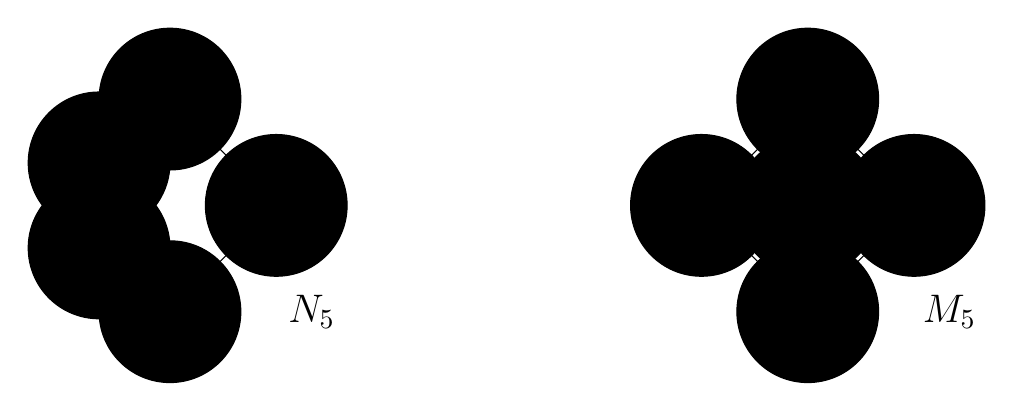
\begin{tikzpicture}[scale=0.9]
\draw (0,0) -- (1.5,1.5) -- (0,3) -- (-1,2.1) -- (-1,.9) -- (0,0);
\foreach \v in {(0,0),(1.5,1.5),(0,3),(-1,2.1),(-1,.9)} \draw[fill=black] \v circle (\tikzvertexsize);
\node at (0,-.5) {\RED{$\mathsf{1}$}};
\node at (-1.6,.9) {\RED{$\mathsf{-1}$}};
\node at (-1.6,2.1) {\RED{$\mathsf{-1}$}};
\node at (2.1,1.5) {\RED{$\mathsf{-1}$}};
\node at (0,3.5) {\RED{$\mathsf{1}$}};
\node at (2,0) {\Large $N_5$};
\begin{scope}[shift={(9,0)}]
\draw (0,0) -- (-1.5,1.5) -- (0,3) -- (1.5,1.5) -- (0,0) -- (0,3);
\foreach \v in {(0,0),(-1.5,1.5),(0,1.5),(1.5,1.5),(0,3)} \draw[fill=black] \v circle (\tikzvertexsize);
\node at (0,-.5) {\RED{$\mathsf{1}$}};
\node at (-2,1.5) {\RED{$\mathsf{-1}$}};
\node at (-.5,1.55) {\RED{$\mathsf{-1}$}};
\node at (2,1.5) {\RED{$\mathsf{-1}$}};
\node at (0,3.5) {\RED{$\mathsf{2}$}};
\node at (2,0) {\Large $M_5$};
\end{scope}
\end{tikzpicture}
\end{center}

And here are $\BB_3$ and another (non-lattice) poset $P$ with the same rank generating function:

\begin{center}
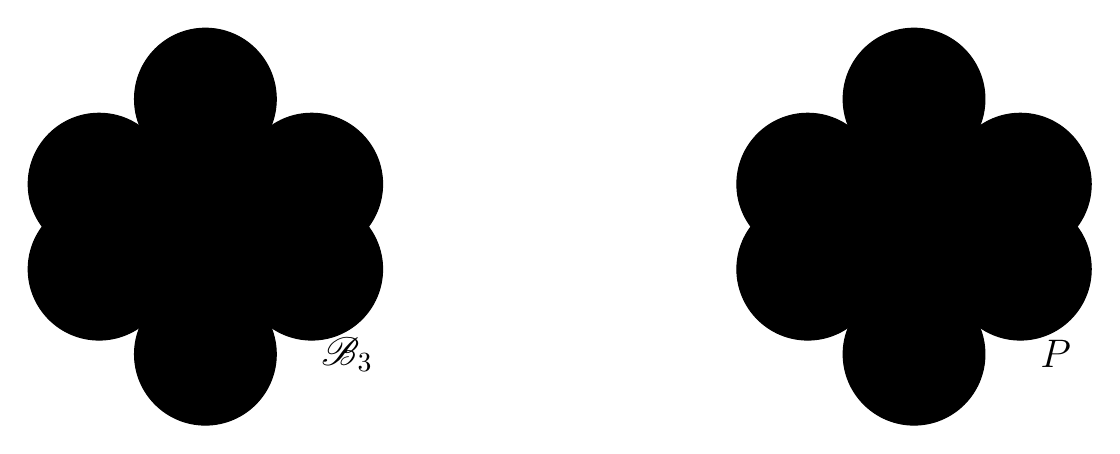
\begin{tikzpicture}[scale=0.9]
\newcommand{\txtshft}{0.6}
\coordinate (Top) at (1,3.6);
\coordinate (AB) at (-.5,2.4);
\coordinate (AC) at (1,2.4);
\coordinate (BC) at (2.5,2.4);
\coordinate (A) at (-.5,1.2);
\coordinate (B) at (1,1.2);
\coordinate (C) at (2.5,1.2);
\coordinate (Bot) at (1,0);
\draw (Top) -- (BC) -- (C) -- (Bot) -- (A) -- (AB) -- (Top) -- (AC) -- (A) -- (AB) -- (B) -- (BC) -- (C) -- (AC);
\draw (Bot) -- (B);
\foreach \v in {Top,AB,AC,BC,A,B,C,Bot} \draw[fill=black] (\v) circle (\tikzvertexsize);
\node at (1-\txtshft,0) {\RED{$\mathsf{1}$}};
\node at (-.5-\txtshft,1.2) {\RED{$\mathsf{-1}$}};
\node at (1-\txtshft,1.2) {\RED{$\mathsf{-1}$}};
\node at (2.5+\txtshft,1.2) {\RED{$\mathsf{-1}$}};
\node at (-.5-\txtshft,2.4) {\RED{$\mathsf{1}$}};
\node at (1+\txtshft,2.4) {\RED{$\mathsf{1}$}};
\node at (2.5+\txtshft,2.4) {\RED{$\mathsf{1}$}};
\node at (1+\txtshft,3.6) {\RED{$\mathsf{-1}$}};
\node at (3,0) {\Large $\BB_3$};

\begin{scope} [shift={(10,0)}]
\coordinate (Top) at (1,3.6);
\coordinate (AB) at (-.5,2.4);
\coordinate (AC) at (1,2.4);
\coordinate (BC) at (2.5,2.4);
\coordinate (A) at (-.5,1.2);
\coordinate (B) at (1,1.2);
\coordinate (C) at (2.5,1.2);
\coordinate (Bot) at (1,0);
\draw (Top) -- (BC) -- (C) -- (Bot) -- (A) -- (AB) -- (Top) -- (Bot);
\draw (AC) -- (A) -- (BC) -- (B);
\foreach \v in {Top,AB,AC,BC,A,B,C,Bot} \draw[fill=black] (\v) circle (\tikzvertexsize);
\node at (1-\txtshft,0) {\RED{$\mathsf{1}$}};
\node at (-.5-\txtshft,1.2) {\RED{$\mathsf{-1}$}};
\node at (1-\txtshft,1.2) {\RED{$\mathsf{-1}$}};
\node at (2.5+\txtshft,1.2) {\RED{$\mathsf{-1}$}};
\node at (-.5-\txtshft,2.4) {\RED{$\mathsf{0}$}};
\node at (1+\txtshft,2.4) {\RED{$\mathsf{1}$}};
\node at (2.5+\txtshft,2.4) {\RED{$\mathsf{2}$}};
\node at (1+\txtshft,3.6) {\RED{$\mathsf{-1}$}};
\node at (3,0) {\Large $P$};
\end{scope}
\end{tikzpicture}
\end{center}
\end{example}


The M\"obius function is useful in many ways.  It can be used to formulate a more general version of inclusion-exclusion called \emph{M\"obius inversion}.  It behaves nicely under poset operations such as product, and has geometric and topological applications.  Even just the single number $\mu_P(\hatzero,\hatone)$ tells you a lot about a bounded poset $P$.  

\begin{example} \textit{The M\"obius function of a boolean algebra.}
Let $2^{[n]}$ be the boolean algebra of rank~$n$ and let $A\subseteq[n]$.
Then $\mu(\hatzero,A)=(-1)^{|A|}$.  To prove this, induct on $|A|$.  The case $|A|=0$ is clear.  For $|A|>0$, we have
  \begin{align*}
  \mu(\hatzero,A) = -\sum_{B\subsetneq A}(-1)^{|B|} &= -\sum_{k=0}^{|A|-1} (-1)^k\binom{|A|}{k} \quad\text{(by induction)}\\
    &= (-1)^{|A|} - \sum_{k=0}^{|A|} (-1)^k\binom{|A|}{k}\\
    &= (-1)^{|A|} - (1-1)^{|A|} ~=~ (-1)^{|A|}.
  \end{align*}

More generally, if $B\subseteq A$, then $\mu(B,A)=(-1)^{|B\sm A|}$,
because every interval of $2^{[n]}$ is a Boolean algebra.
\end{example}

The M\"obius function behaves nicely with respect to direct products of posets, for the following reason.
Let $P,Q$ be bounded finite posets.  For $\alpha\in I(P)$ and $\phi\in I(Q)$, define $\alpha\phi\in I(P\x Q)$ by
\[\alpha\phi[(x,x'),(y,y')] = \alpha(x,y)\phi(x',y').\]
This defines a linear transformation $I(P)\otimes I(Q)\to I(P\x Q)$.

\begin{proposition}\label{incidence-product}
The map $I(P)\otimes I(Q)\to I(P\x Q)$ just defined is an algebra homomorphism: for all
$\alpha,\beta\in I(P)$ and $\phi,\psi\in I(Q)$, we have
\[\alpha\phi*\beta\psi = (\alpha*\beta)(\phi*\psi).\]
Furthermore, the incidence functions $\delta$, $\zeta$ and $\mu$ are multiplicative on direct products, i.e.,
\[\delta_{P\x Q}=\delta_P\delta_Q, \qquad \zeta_{P\x Q}=\zeta_P\zeta_Q,\qquad \mu_{P\x Q}=\mu_P\mu_Q.\]
\end{proposition}

\begin{proof} Let $(x,x')$ and $(y,y')$ be elements of $P\x Q$.  Then
\begin{align*}
(\alpha\phi*\beta\psi) [(x,x'),(y,y')]
&= \sum_{(z,z')\in[(x,x'),(y,y')]} \alpha\phi[(x,x'),(z,z')]\cdot\beta\psi[(z,z'),(y,y')]\\
&= \sum_{z\in[x,y]} \sum_{z'\in[x',y']} \alpha(x,z)\phi(x',z')\beta(z,y)\psi(z',y')\\
&= \left[\sum_{z\in[x,y]}\alpha(x,z)\beta(z,y)\right] \left[\sum_{z'\in[x',y']} \phi(x',z') \psi(z',y')\right]\\
&= (\alpha*\beta(x,y))\cdot(\phi*\psi(x',y')).
\end{align*}
Multiplicativity of $\delta$ and $\zeta$ is immediate from their definitions.  Also,
\[\zeta_{P\x Q}*\mu_P\mu_Q = \zeta_P\zeta_Q*\mu_P\mu_Q = (\zeta_P*\mu_P)(\zeta_Q*\mu_Q) = \delta_P\delta_Q = \delta_{P\x Q}\]
which says that $\mu_P\mu_Q = \zeta_{P\x Q}^{-1} = \mu_{P\x Q}$.
(It is also possible to prove that $\mu_P\mu_Q = \mu_{P\x Q}$ directly from the definition.)
\end{proof}

\begin{example}
Let $P$ be a product of $n$ chains
of lengths $a_1,\dots,a_n$.  That is,
\[P = \{x=(x_1,\dots,x_n) \st 0\leq x_i \leq a_i \text{ for all } i \in[n]\},\]
ordered by $x\leq y$ iff $x_i\leq y_i$ for all $i$.  Then
\[\mu(\hatzero,x) = \begin{cases}
    0 & \text{ if $x_i\geq 2$ for at least one $i$;}\\
    (-1)^s & \text{ if $x$ consists of $s$ 1's and $n-s$ 0's.}
\end{cases}\]
(The Boolean algebra is the special case that $a_i=2$ for every $i$.)  This conforms
to the definition of M\"obius function that you may have seen in Math~724.  This formula
is sufficient to calculate $\mu(y,x)$ for all $x,y\in P$, because every interval
$[y,\hatone]\subseteq P$ is also a product of chains.
\end{example}

Here are a couple of enumerative applications of the M\"obius function.

\begin{theorem}[Philip Hall's Theorem] \cite[Prop.~3.8.5]{EC1-Ed2}
Let $P$ be a finite bounded poset with at least two elements.  For $k\geq 1$, let
\[c_k = c_k(P) = \Big|\{\hatzero=x_0<x_1<\cdots<x_k=\hatone\}\Big|\]
be the number of chains of length~$i$ between $\hatzero$ and $\hatone$.  Then
\[\mu_P(\hatzero,\hatone)=\sum_k (-1)^k c_k.\]
\end{theorem}

\begin{proof}
Recall that $c_k=\eta^k(\hatzero,\hatone)=(\zeta-\delta)^k(\hatzero,\hatone)$.
The trick is to use the geometric series expansion $1/(1+h)=1-h+h^2-h^3+h^4-\cdots$.  Clearing both denominators and replacing $h$ with $\eta$ and 1 with $\delta$, we get
%\[\delta=(\delta+\eta)\left(\sum_{k=0}^\infty(-1)^k\eta^k\right)\]
%where 1 means $\delta$ (the multiplicative unit in $I(P)$).
%Since sufficiently high powers of $\eta$ vanish,
%this is a perfectly good equation of polynomials in $I(P)$.  Therefore,
\[(\delta+\eta)^{-1} = \left(\sum_{k=0}^\infty(-1)^k\eta^k\right).\]
This is a valid equation in $I(P)$, because $\eta^k=0$ for $k$ sufficiently large.
Evaluating both sides on $[\hatzero,\hatone]$ gives
\[
\sum_{k=0}^\infty (-1)^k c_k ~=~ \sum_{k=0}^\infty (-1)^k\eta^k(\hatzero,\hatone) ~=~ (\delta+\eta)^{-1}(\hatzero,\hatone) ~=~ \zeta^{-1}(\hatzero,\hatone) ~=~ \mu(\hatzero,\hatone).\qedhere
\]
\end{proof}

This alternating sum looks like an Euler characteristic.  In fact it is.
%Define the \defterm{order complex} $\Delta(P)$ of a poset $P$ to
%be the simplicial complex on vertices~$P$ whose faces are the chains
%of $P$.  (Note that this is a simplicial complex because every subset
%of a chain is a chain.)  Then $c_k(P)=f_{k-2}(\Delta(P))$, so
%$\mu_{\hat P}(\hatzero,\hatone)=\tilde\chi(\Delta(P))$, the reduced Euler
%characteristic (see Exercise~\ref{euler-poincare}).

\begin{corollary}
Let $P$ be a finite bounded poset with at least two elements, and let $\Delta(P)$ be its \emph{order complex}, i.e., the simplicial complex whose vertices are the elements of $P\sm\{\hatzero,\hatone\}$ and whose simplices are chains.  Each chain $x_0=\hatzero<x_1<\cdots<x_k=\hatone$ gives rise to a simplex $\{x_1,\dots,x_{k-1}\}$ of $\Delta(P)$ of dimension $k-2$.  Hence $f_{k-2}(\Delta(P))=c_k(P)$ for all $k\geq1$, and the reduced Euler characteristic of $\Delta(P)$ is
\[\tilde\chi(\Delta(P))~\eqdef~\sum_{k\geq-1} (-1)^k f_k(\Delta(P))=\sum_{k\geq1} (-1)^{k-2} c_k(P)\mu_P(\hatzero,\hatone).\eqno\qed\]
\end{corollary}




\begin{example}
For the poset $P$ of Example~\ref{moebius-ex}, we have $c_0=0$, $c_1=1$, $c_2=6$, $c_3=6$, and $c_k=0$ for $k>3$.  So $c_0-c_1+c_2-c_3=-1=\mu_P(\hatzero,\hatone)$.
\end{example}

\end{document}